
%%%%%%%%%%%%%%%%%%%%%%%%%%%%%%%%%%%%%%%%%%%%%%%%%%%%%%%%%%%%%
\frame{
\frametitle{Type of resampling}

\begin{itemize}

\item  \textbf{Randomization exact test} (or permutation test) developed by R. A. Fisher (1935/1960), the founder of classical statistical testing.

\

 \item  \textbf{Jackknife} invented by Maurice Quenouille (1949) and later developed by John W. Tukey (1958). 
% first purpose of Jackknife is to detect outliers

\

 \item \textbf{Bootstrap}  invented by Bradley Efron (1979, 1981, 1982) and further developed by Efron and Tibshirani (1993). 

\

 \item \textbf{Cross-validation} 

\end{itemize}
}
%%%%%%%%%%%%%%%%%%%%%%%%%%%%%%%%%%%%%%%%%%%%%%%%%%%%%%%%%%%%%%%
\frame{
\frametitle{Resampling}

\begin{definition}
\alert{Resampling} means that the inference is based upon repeated sampling within the same sample.
Resampling is tied to the Monte Carlo simulation. Some may distinguish both in that resampling consider all possible replications (permutation test, jackknife) and the Monte-Carlo sampling restrict the resampling to a certain number of replications (bootstrap, randomisation test). 
\end{definition}

Another difference in between resampling methods  is  the nature of the  resamples: computed with or without replacement.


}
%%%%%%%%%%%%%%%%%%%%%%%%%%%%%%%%%%%%%%%%%%%%%%%%%%%%%%%%%%%%%%%
\frame{
\frametitle{Introduction to cross-validation}

\begin{itemize}
\item \textbf{Cross-validation} was proposed by Kurtz (1948-simple cross-validation) , extended by Mosier (1951-double cross-validation) and  by Krus and Fuller  (1982-  multicross-validation).

\

\item The original objective of cross-validation is to verify replicability of results.

\

\item Similarly with hypothesis testing, the goal is to find out if the result is replicable or just a matter of random. 


\end{itemize}


}
%%%%%%%%%%%%%%%%%%%%%%%%%%%%%%%%%%%%%%%%%%%%%%%%%%%%%%%%%%%%%%%
\frame{
\frametitle{prediction error}

\begin{definition}
A \alert{prediction error} measures how well a model predicts the response value of a future observation. It is often used for model selection.

It is defined as:
\begin{itemize}
\item the expected square difference between a future response and the prediction from the model in regression models:
$$
\mathbb{E}(y-\hat{y})
$$
\item the probability of incorrect classification in classification problem: 
$$
\pmb{\mathcal{P}}(y \neq \hat{y})
$$
\end{itemize}
\end{definition}
}
%%%%%%%%%%%%%%%%%%%%%%%%%%%%%%%%%%%%%%%%%%%%%%%%%%%%%%%%%%%%%%%
\frame{
\frametitle{The linear regression model}
\begin{itemize}
\item We have a set of (2-dimensional) points $z =\lbrace (x_i,y_i) \rbrace_{i=1,\cdots,n}$. 
\item An unknow relation is linking $y_i$ to $x_i$ such as:
$$
\begin{array}{ll}
y_i&=\beta(x_i)+\epsilon_{i}\\
&\\
&=\sum_{q=0}^{p} \beta_q \ x_i^q+\epsilon_{i}\\
\end{array} 
$$
\item The error terms  $\epsilon_{i}$ are assumed to be random sample from a random distribution having expectation 0 and variance $\sigma^2$.


\end{itemize}



}
%%%%%%%%%%%%%%%%%%%%%%%%%%%%%%%%%%%%%%%%%%%%%%%%%%%%%%%%%
\frame{
\frametitle{The Model Selection Problem}

\begin{figure}[!h]
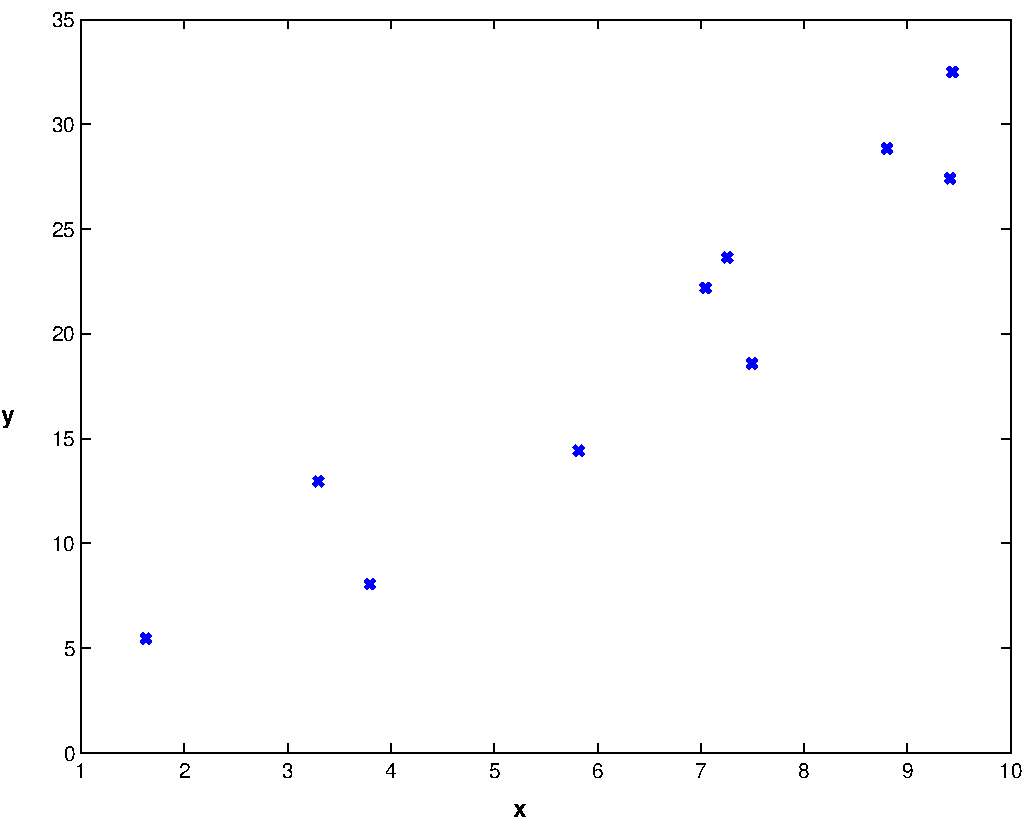
\includegraphics[width=.45\linewidth]{datacv}
\caption{Exemple of data set ( In this example $(\beta_0,\beta_1,\beta_2)=(1,3,0)$, $\sigma=3$ and $n=10$).}
\end{figure}

}
%%%%%%%%%%%%%%%%%%%%%%%%%%%%%%%%%%%%%%%%%%%%%%%%%%%%%%%%%
\frame{
\frametitle{The Model Selection Problem}

\begin{figure}[!h]
\begin{tabular}{cc}
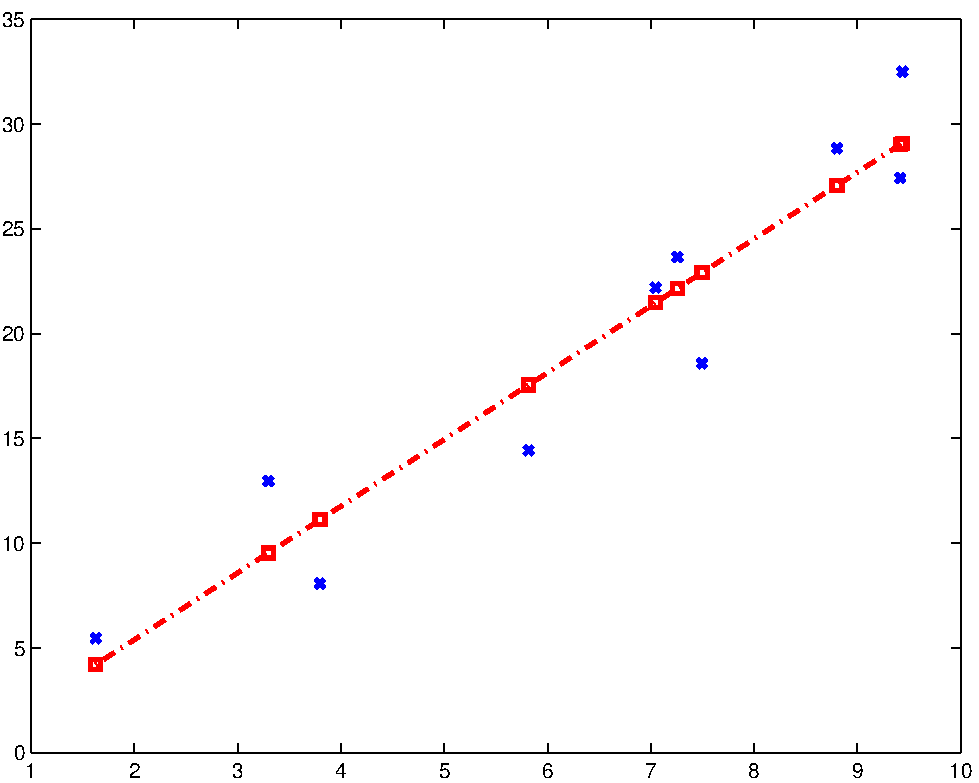
\includegraphics[width=.45\linewidth]{datacvline}&
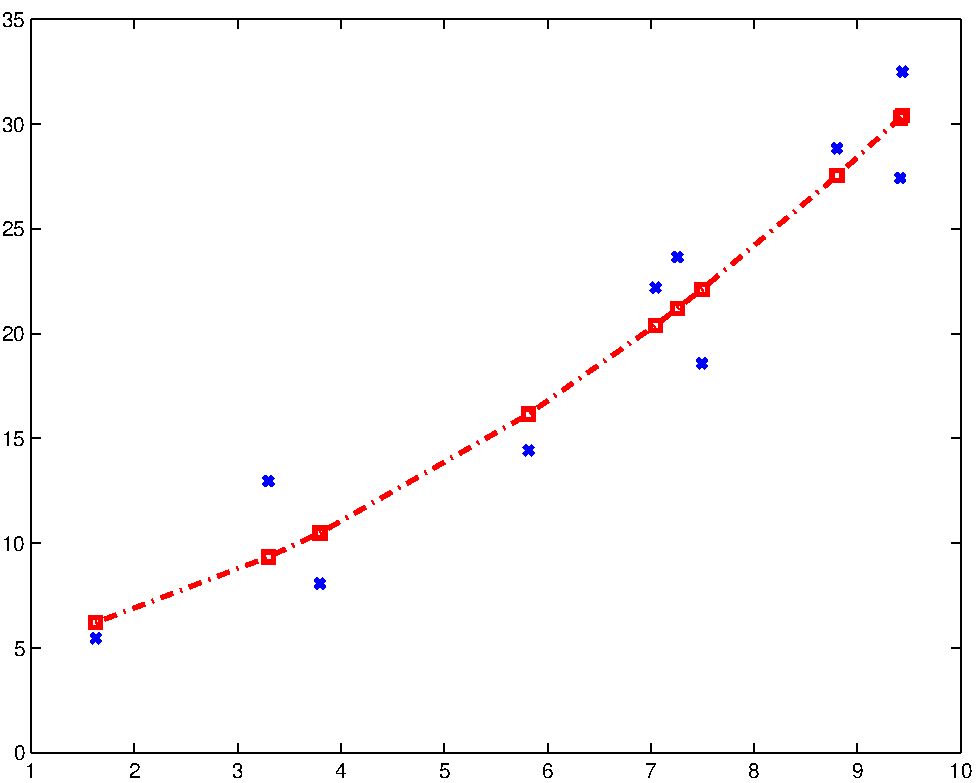
\includegraphics[width=.45\linewidth]{datacvquad}\\
Model A:  $\hat{y}=\hat{\beta}_1\ x+\hat{\beta}_0$ & Model B:  $\hat{y}=\hat{\beta}_2\  x^2+\hat{\beta}_1\  x+\hat{\beta}_0$ \\
\end{tabular}
\caption{The data points (blue cross) fitted assuming a linear model (left), and a quadratic model (right). Regression estimates are  $(\hat{\beta}_0,\hat{\beta}_1)=(-0.9802, 3.1866)$ for model A, and  $(\hat{\beta}_0,\hat{\beta}_1,\hat{\beta}_2)=(4.2380,0.8875, 0.1997)$ for model 2. \alert{Which model is the best ?}}
\end{figure}
}
%%%%%%%%%%%%%%%%%%%%%%%%%%%%%%%%%%%%%%%%%%%%%%%%%%%%%%%

%%%%%%%%%%%%%%%%%%%%%%%%%%%%%%%%%%%%%%%%%%%%%%%%%%%%%%%
\frame{
\frametitle{The Model Selection Problem}

\begin{itemize}
\item \alert{Which model is the best ?} = How well are you going to predict
future data drawn from the same
distribution?

\item As a prediction error, we can compute the average Residual Squared Error (RSE):
$$
\mathrm{PE} = \quad \frac{\mathrm{RSE}}{n}=\frac{\sum_{i=1}^{n} (y_i-\hat{y}_i)^2}{n}
$$
where $\hat{y}_i$ is the prediction by the model $\hat{y}_i=\hat{\beta}(x_i)$.

\item To start, $y_i$ is taken in the sample $\mathbf{z}$ (instead of a future response). In this case, the prediction error  is then called the \alert{apparent prediction error (APE)}  
\end{itemize}

}
%%%%%%%%%%%%%%%%%%%%%%%%%%%%%%%%%%%%%%%%%%%%%%%%%%%%%%%
\frame{
\frametitle{The Model Selection Problem}

\begin{figure}[!h]
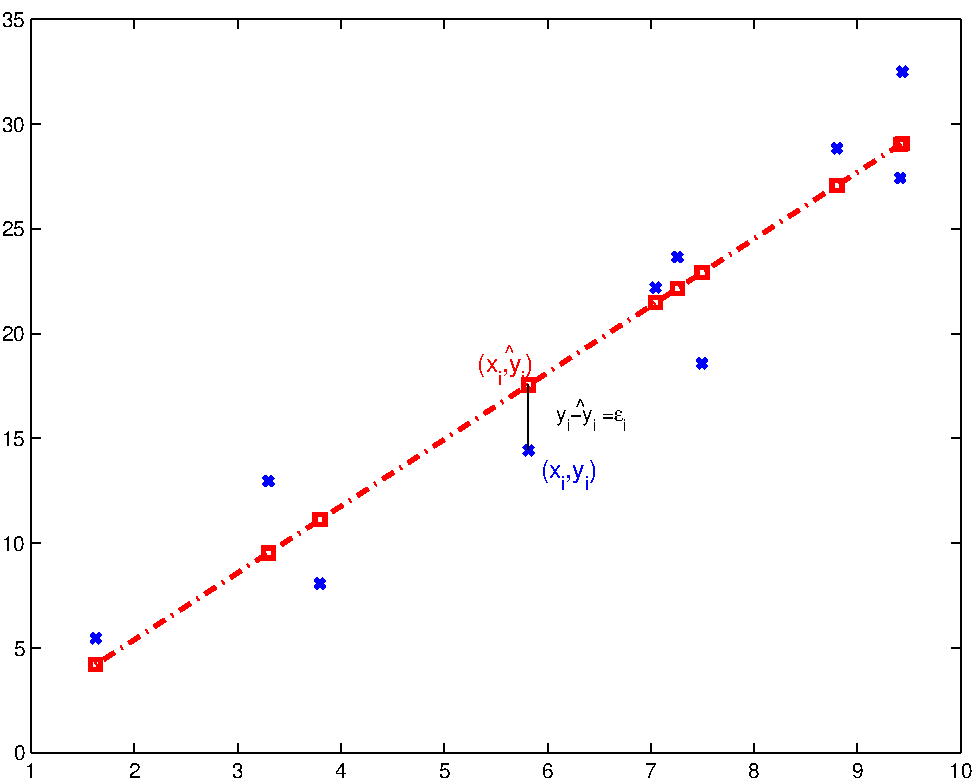
\includegraphics[width=.8\linewidth]{datacvlineb}
\end{figure}
}
%%%%%%%%%%%%%%%%%%%%%%%%%%%%%%%%%%%%%%%%%%%%%%%%%%%%%%%
\frame{
\frametitle{The Model Selection Problem}

For our two models:
\begin{itemize}

\item For model A,  the apparent prediction error is $7.1240$.

\item For model B, the apparent prediction error is $5.8636$

\end{itemize}

The apparent prediction error computed with model B is better (smaller) than
with the model A. Note that  the family of functions in B contains the ones defined in A. So B can capture more   variabilities in the data set $\mathbf{z}$, and can fit (in the sense of the APE)  better the observation $\mathbf{z}$.

\begin{itemize}

\item  But this is an \textit{apparent} prediction error. What is the prediction error for a new observation ? 

\item \alert{How to get a new sample to compute this prediction?}
\end{itemize}
}


%%%%%%%%%%%%%%%%%%%%%%%%%%%%%%%%%%%%%%%%%%%%%%%%%%%%%%%
\frame{
\frametitle{Cross-validation}

\begin{itemize}
\item For a more realistic estimate of the prediction error, we need a test sample different from the   training sample.

\

\item One way is to split the observation $\mathbf{z}$ into two sets, one for training and the other one for testing. 

\
\item Using  a part of the available observation to fit the model, and a different part to test in the computation of predication error is known as the cross-validation.  


\end{itemize}

}
\frame{
\frametitle{Simple and double cross-validation}

\begin{itemize}
\item \textbf{Simple cross-validation}. Divide the set $\mathbf{z}$ into two groups, one for \textit{training} and the other one for \textit{testing}. The parameters $\beta$ are estimated on the training data set. The cross-validation  is the prediction error  computed using the test sample.

\

\item \textbf{Double cross-validation}.  Models are generated for  both sub-samples, and then both equations are used to generate  cross-validation.

\end{itemize}

}
%%%%%%%%%%%%%%%%%%%%%%%%%%%%%%%%%%%%%%%%%%%%%%%%%%%%%%%
\frame{
\frametitle{K-Fold cross-validation}

\begin{beamercolorbox}[wd=\linewidth, rounded=true,shadow=true]{postit}
\begin{enumerate}
\item Split $\mathbf{z}$ into $K$ equal subsets $\mathbf{z}_k$

\

\item  Do $K$ times:
\begin{itemize}
\item Estimate the model $\beta_{(k)}$ on $\mathbf{z}_{(k)}=\lbrace \mathbf{z}_1, \cdot,\mathbf{z}_{k-1}, \mathbf{z}_{k+1}, \cdots,\mathbf{z}_{K} \rbrace $ 

\

\item Compute the prediction error $\mathrm{PE}(k)$ between the  test sample $\mathbf{z}_k$ and the predicted model by $\beta_{(k)}$.
\end{itemize}

\

\item Compute the  average of those $K$ prediction errors as the overall estimate of the prediction error 
$$
\mathrm{CV}=\frac{1}{K} \sum_{k=1}^{K} \mathrm{PE}(k)
$$
\end{enumerate}
\end{beamercolorbox}
}
%%%%%%%%%%%%%%%%%%%%%%%%%%%%%%%%%%%%%%%%%%%%%%%%%%%%%%%
\frame{
\frametitle{K-Fold cross-validation}
\begin{itemize}
\item The number $K$ of subsets depend on the size $n$ of the observation $\mathbf{z}$.

\

  \item For large datasets, even 3-Fold Cross Validation will be quite accurate.

\

\item For small datasets, we may have to use \textbf{leave-one-out} cross validation  where $K=n$.

\ 

\item \textbf{Multicross-validation} is an extension of double cross-validation. Double cross-validation procedures are repeated many times by randomly selecting sub-samples from the data set. 
\end{itemize}
}
%%%%%%%%%%%%%%%%%%%%%%%%%%%%%%%%%%%%%%%%%%%%%%%%%%%%%%%
\frame{
\frametitle{Cross-validation and parameter selection} 
\begin{itemize}
\item We just show how to perform model selection (i.e. choice of the number of parameters $p$ in the regression model).

\

\item Cross-validation can also be used for parameter estimation by  choosing the parameter value  which minimises the prediction error.

\

\item The cross-validation is computed using subsamples of  $\mathbf{z}$. An alternative consists in considering bootstrap samples. 

\end{itemize}
}
%%%%%%%%%%%%%%%%%%%%%%%%%%%%%%%%%%%%%%%%%%%%%%%%%%%%%%%
\frame{
\frametitle{Bootstrap estimates of the prediction error}


\begin{beamercolorbox}[wd=\linewidth, rounded=true,shadow=true]{postit}
\begin{enumerate}
\item Compute $B$ boostrap resamples $\mathbf{z}^{*}$ from the observation $\mathbf{z}$

\

\item Compute the model parameter $\beta^{*(b)}$ from  $\mathbf{z}^{*}$, and the corresponding prediction error PE$(b)$ with the testing observation being the original sample $\mathbf{z}$. 

\

\item Compute the  average of those $B$ prediction errors as the overall estimate of the prediction error 
$$
\mathrm{CV}_{boot}=\frac{1}{B} \sum_{b=1}^{B} \mathrm{PE}(b)
$$
\end{enumerate}
\end{beamercolorbox}

}
%%%%%%%%%%%%%%%%%%%%%%%%%%%%%%%%%%%%%%%%%%%%%%%%%%%%%%
\frame{
\frametitle{Bootstrap estimates of the prediction error}

\begin{itemize}
\item This bootstrap extension to cross-validation turns out to not work very well. But it can be improved.
 
\item Keep the record of the results from the previous procedure. Run a second experiment but choosing the bootstrap sample $\mathbf{z}^{*}$ itself as a test sample. Compute the difference of the two previous results (this difference is called optimism). This optimism is then added to the APE ( as a bias correction).

\item Which is best between CV and bootstrap alternatives is not really clear. 

\end{itemize}
}


%%%%%%%%%%%%%%%%%%%%%%%%%%%%%%%%%%%%%%%%%%%%%%%%%%%%%%
\frame{
\frametitle{Other estimates of  the prediction error}

\begin{itemize}
\item So far, we have define the PE using the average RSE. This is the prediction error measure used in cross-validation.

\item One can think of using other measures such as the  Bayesian Information Criterion (BIC)
$$
\frac{RSE}{n}+\log{n} \cdot p\hat{\sigma}^{2}/n 
$$

\item BIC penalises the model as  the number of parameter $p$ increases. It is a consistent criterion i.e. it chooses the good model as $n\rightarrow \infty$.

\item However, two drawbacks of the BIC compared to CV:
\begin{itemize}
\item you need an estimate  $\hat{\sigma}$.
\item you need the knowledge of $p$. 
\end{itemize} 

\end{itemize}
}
%%%%%%%%%%%%%%%%%%%%%%%%%%%%%%%%%%%%%%%%%%%%%%%%%%%%%%%
\frame{
\frametitle{Summary}

\begin{itemize}
\item Cross validation method applied to selection model (regression).

\

\item Other applications such as classification use the cross-validation. In this case, $y_i$ is a label  indicating the class. The prediction error is defined as a misclassification rate.   

\

\item Those methods  are very much used  in machine learning.
% (= area of artificial intelligence concerned with the development of techniques which allow computers to learn). 
% It is a method for creating computer programs by the analysis of data sets. It is also concerned with the algorithmic complexity of computational implementations. 


\end{itemize}

}
